\documentclass[slides,compress]{beamer}
\usepackage{graphicx,amsmath,hyperref}
\usepackage{verbatim}

\usepackage[normalem]{ulem}

\usetheme{default}
\useinnertheme{rectangles}

\title{\huge You can't get the staff - an electronic alternative...}
\subtitle{\large (an introduction to xia2)}

\author{Graeme Winter}
\institute{Diamond Light Source}
\date{CCP4 Study Weekend 2012}

\begin{document}

\setbeamertemplate{background}{

\includegraphics[width=\paperwidth,height=\paperheight]
{diamond-background.png}
}

\frame{\maketitle}

\frame{
\frametitle{Overview}
\begin{itemize}
\item{Background}
\item{What is xia2?}
\item{What does it do and how do I use it?}
\item{What decisions does it make?}
\item{Conclusions / summary}
\end{itemize}
}

\section{Background}

\begin{frame}
\frametitle{Before we start...}
\begin{itemize}
\item{No 
MOSFLM \footnote{A.G.W. Leslie, Acta Cryst. (2006) D62, 48-57},
XDS\footnote{W. Kabsch, Acta Cryst. (2010) D66, 125-132}, 
SCALA\footnote{P. Evans, Acta Cryst. (2006) D62, 72-82}, 
CCP4\footnote{CCP4, Acta Cryst. (1994) D50, 760-763}
}
\item{$\rightarrow$ no xia2}
\item{No 
LABELIT\footnote{N.K. Sauter et al.
J. Appl. Cryst. (2004) 37, 399-409},
CCTBX\footnote{R.W. Grosse-Kunstleve et al.
J. Appl. Cryst. (2002) 35, 126-136},
POINTLESS\footnote{P. Evans, Acta Cryst. (2006) D62, 72-82}, 
etc.}
\item{$\rightarrow$ harder to write xia2, less reliable}
\end{itemize}
\end{frame}

\begin{frame}
\frametitle{Acknowledgements}
\begin{itemize}
\item{Andrew Leslie, Harry Powell, Phil Evans, Wolfgang Kabsch, Kay Diederichs,
Nick Sauter, Ralf Grosse-Kunstleve}
\item{Alun Ashton, Dave Stuart, Diamond beamline staff, Miroslav Papiz, 
Steve Prince, Colin Nave, xia2 users, providers of test data (esp. JCSG)}
\item{Funding from Diamond Light Source, BBSRC e-Science e-HTPX project, 
BioXHit}
\end{itemize}
\end{frame}

\begin{frame}
\frametitle{Background}
\begin{itemize}
\uncover<1->{
\item{Comprehensive, trusted software available}
\item{Background of strong publications (esp. CCP4 study weekends)}
\item{Massive advances in computing}
\item{New synchrotron for UK}
}
\uncover<2->{
\item{$\rightarrow$ a great time to develop automated data reduction}
}
\end{itemize}
\end{frame}

\section{What is xia2?}

\begin{frame}
\frametitle{What is xia2?}
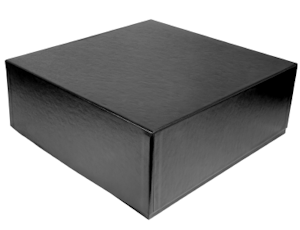
\includegraphics[scale=1]{figures/blackbox.png}
\end{frame}

\begin{frame}
\frametitle{What is xia2?}
{\large
\uncover<1->{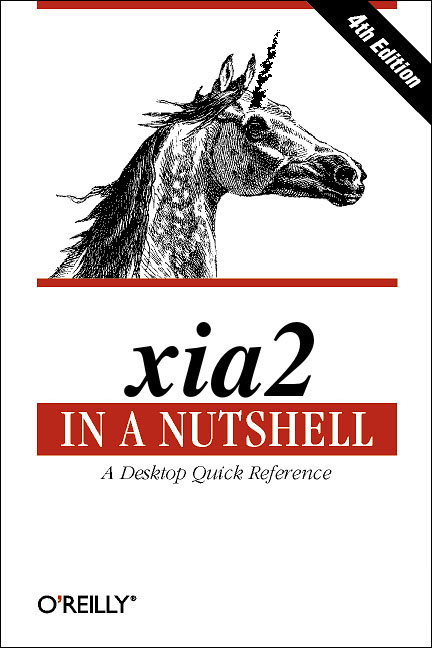
\includegraphics[scale=0.125]{figures/xia2-in-a-nutshell.jpg}}
\uncover<2->{
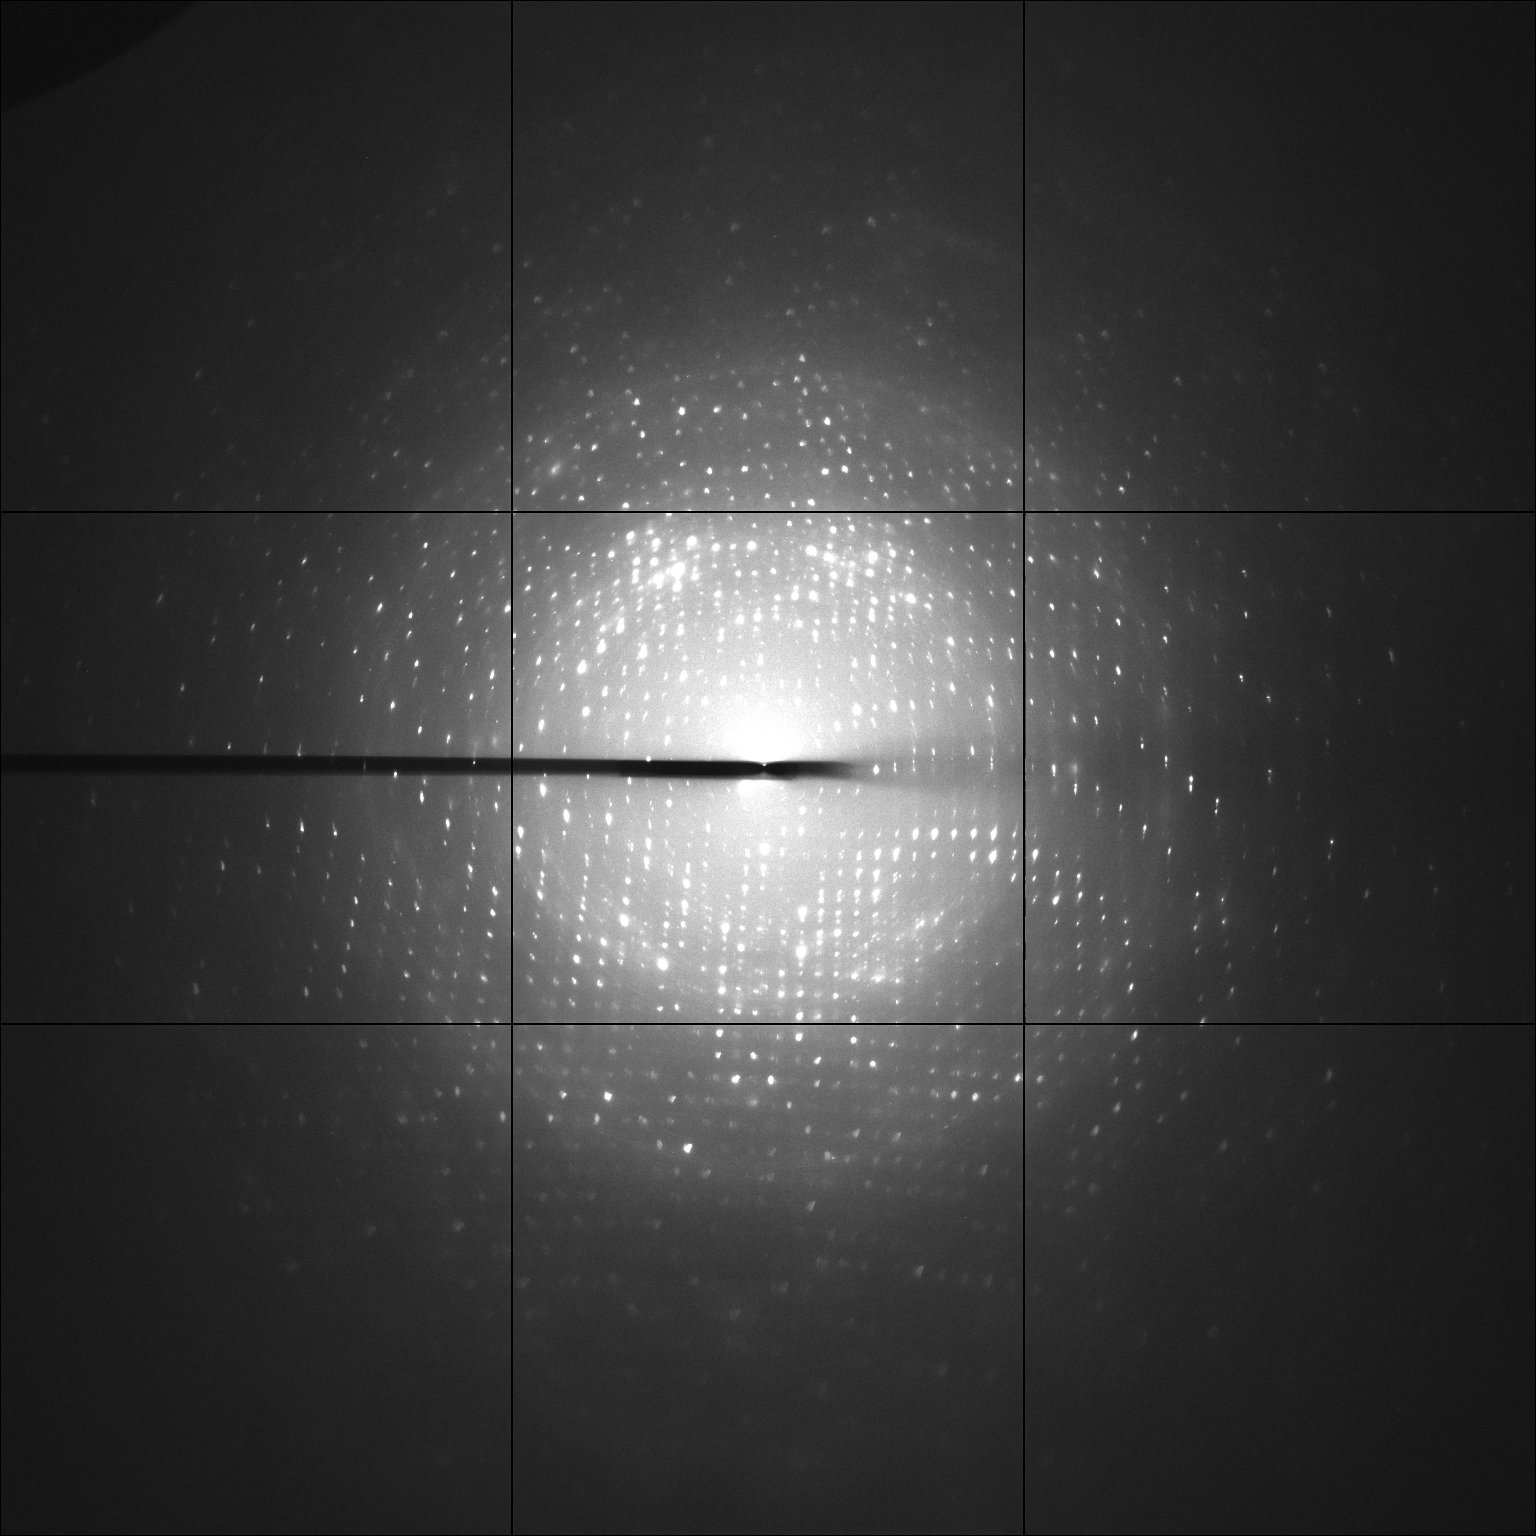
\includegraphics[scale=0.05]{figures/example-diffraction-image-small.jpg} 
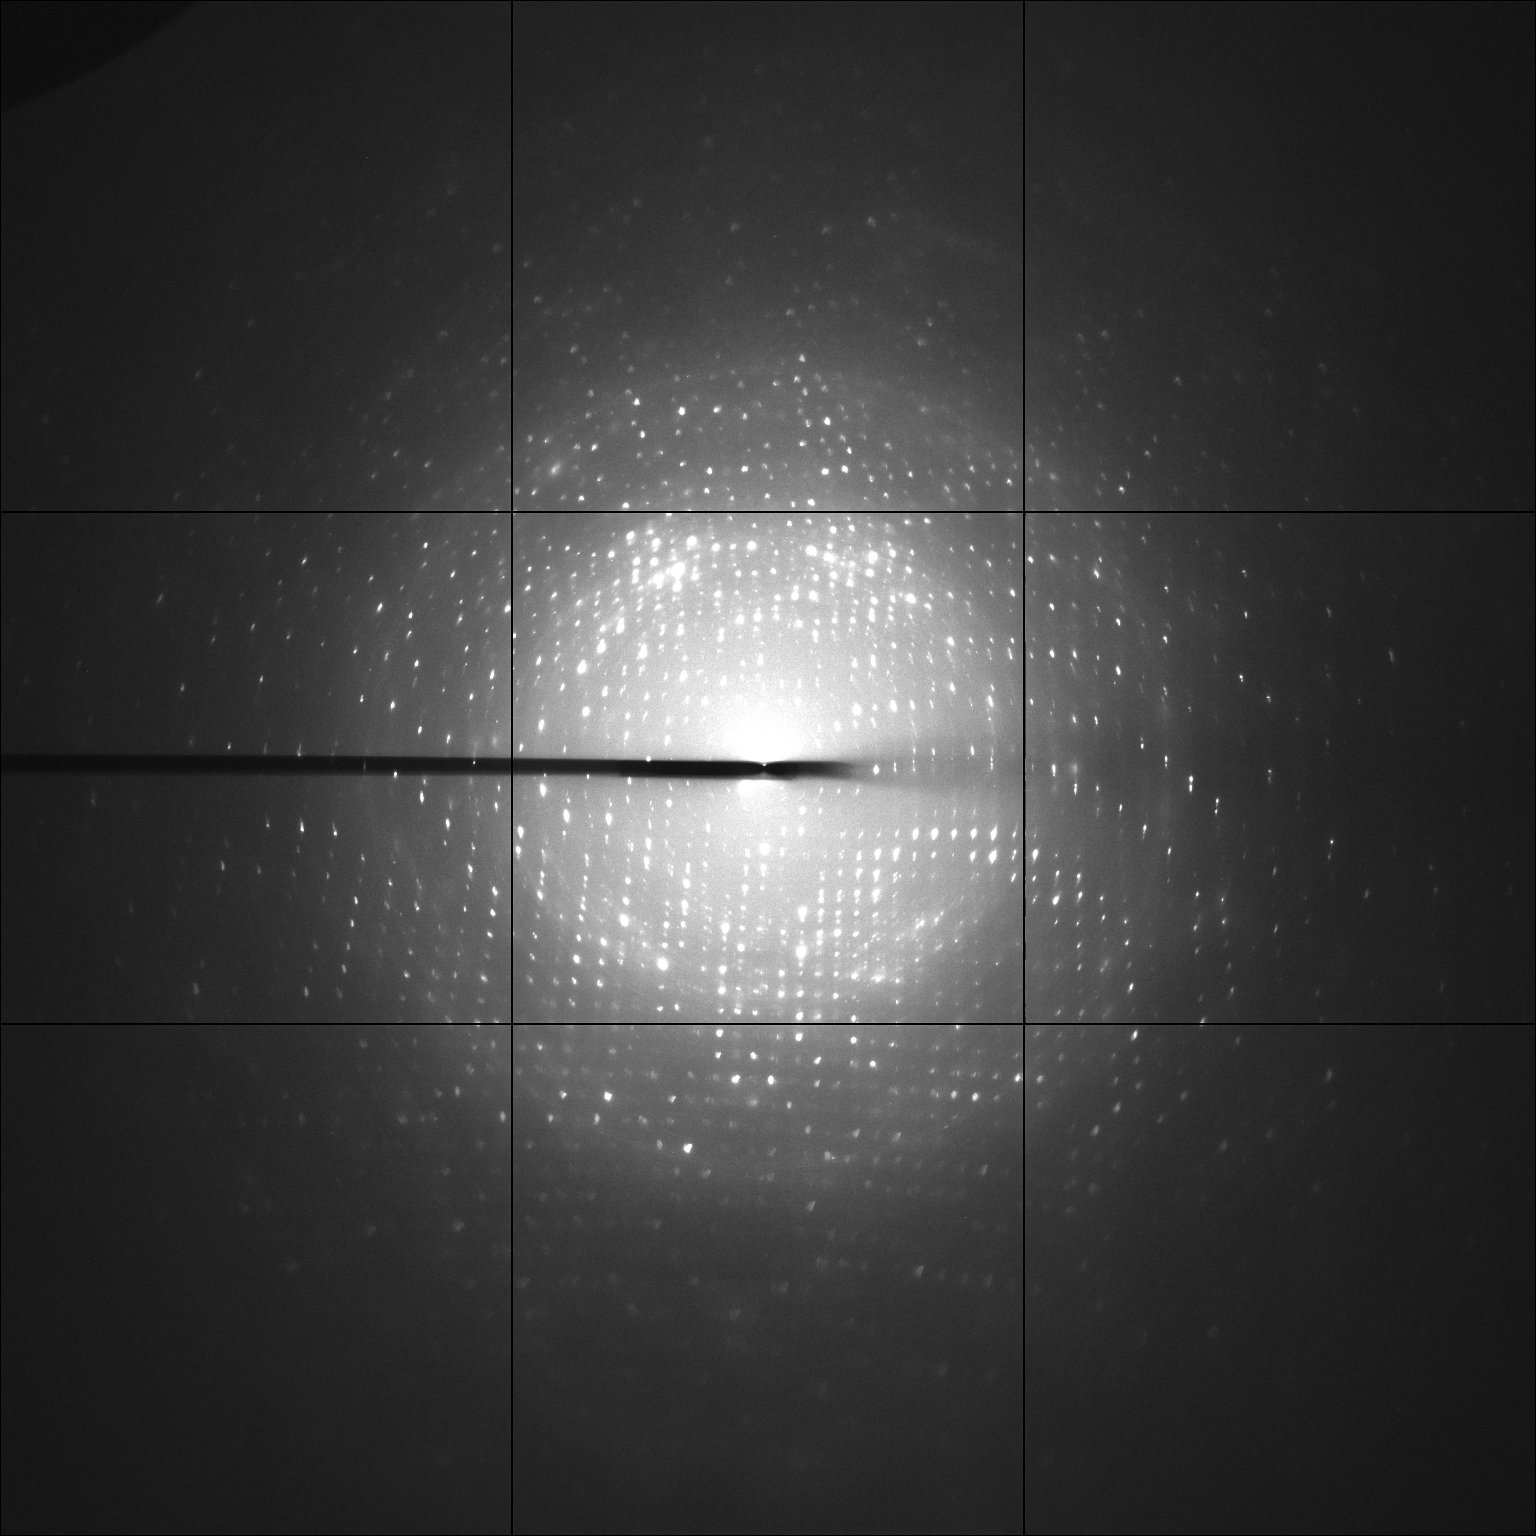
\includegraphics[scale=0.05]{figures/example-diffraction-image-small.jpg}
}
\uncover<3->{$\rightarrow H K L I \sigma_{I}$}
}
\end{frame}

\begin{frame}
\frametitle{What is xia2?}
\begin{itemize}
\uncover<1->{
\item{An \emph{expert} system to perform diffraction data and processing on 
your behalf using your software}
}
\uncover<2->{
\item{A system which can correctly handle multi-pass, multi-wavelength data
sets}
}
\uncover<3->{
\item{\emph{Not} a data processing package}
}
\end{itemize}
\end{frame}

\begin{frame}
\frametitle{Why ``you can't get the staff?''}
\begin{itemize}
\item{12 datasets / hour possible}
\item{Limited help}
\item{Human endurance}
\item{Intended xia2 as tool to delegate data processing to}
\end{itemize}
\end{frame}

\begin{frame}
\frametitle{Why is this useful?}
\begin{itemize}
\item{Second opinion}
\item{Allows you to focus on problem cases}
\item{Help  busy / novice users}
\item{Provides access to other tools}
\item{Reproducible processing}
\end{itemize}
\end{frame}

\section{Using xia2}

\begin{frame}
\frametitle{Using xia2}
%{\centerline
\begin{tabular}{c}
{\huge
xia2 -2d /here/are/my/data
}\\
\\
{\huge \emph{- or -}} \\
\\
{\huge
xia2 -3d /here/are/my/data
}\\
\end{tabular}
%}
\end{frame}

\begin{frame}
\frametitle{Sorry...}
\uncover<1-2>{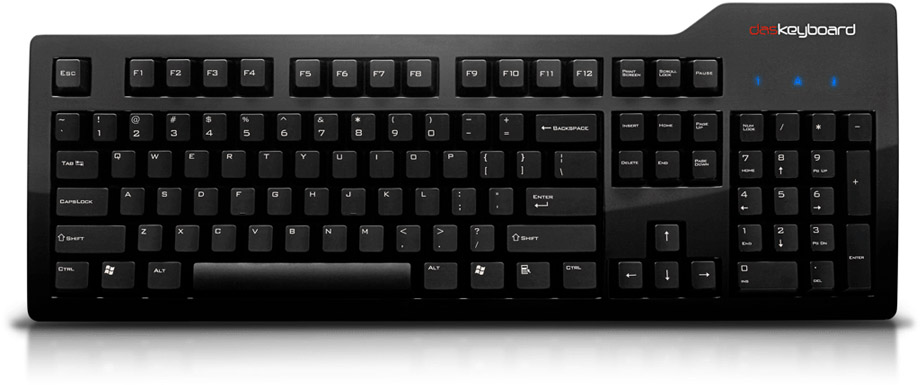
\includegraphics[scale=0.1]{figures/keyboard.jpg}}
\uncover<2-2>{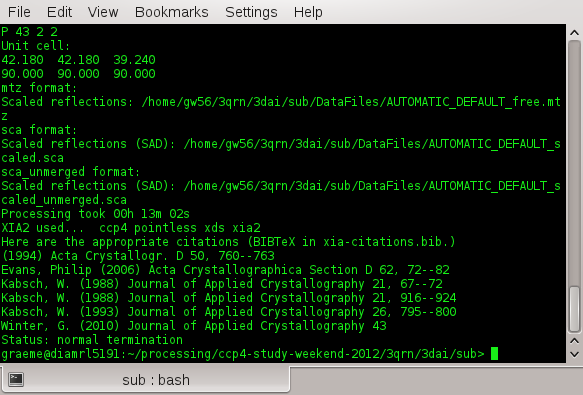
\includegraphics[scale=0.15]{figures/terminal.png}}
\uncover<3->{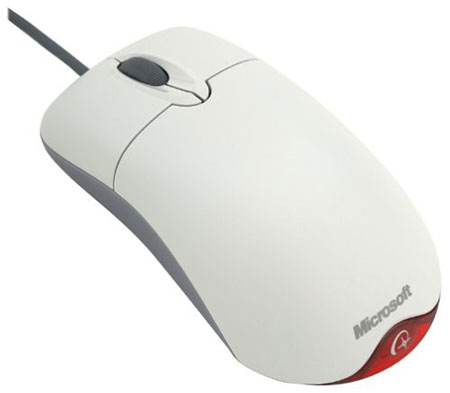
\includegraphics[scale=0.15]{figures/mouse.jpg}}
\end{frame}

\begin{frame}
\frametitle{Options (1)}
\begin{itemize}
\item{-atom X - tell xia2 to separate anomalous pairs}
\end{itemize}
\end{frame}

\begin{frame}
\frametitle{How does it figure what to do?}
\begin{itemize}
\uncover<1->{\item{Read all of the image headers then}}
\uncover<2->{\item{Organise these into sweeps then}}
\uncover<2->{\item{Organise these into wavelengths then}}
\uncover<2->{\item{Assign all of these wavelengths to a crystal}}
\end{itemize}
\end{frame}

\begin{frame}
\frametitle{How does it figure what to do?}
\hspace{3cm}
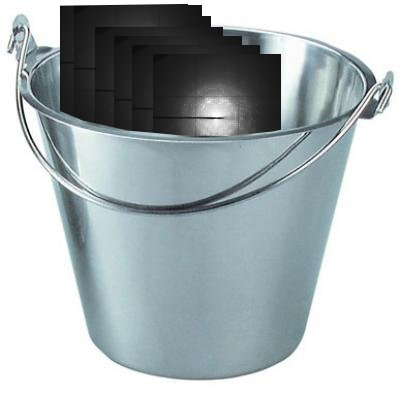
\includegraphics[scale=0.4]{figures/bucket-of-images.jpg}
\end{frame}

\begin{frame}
\frametitle{How does it figure what to do?}
\hspace{4cm}
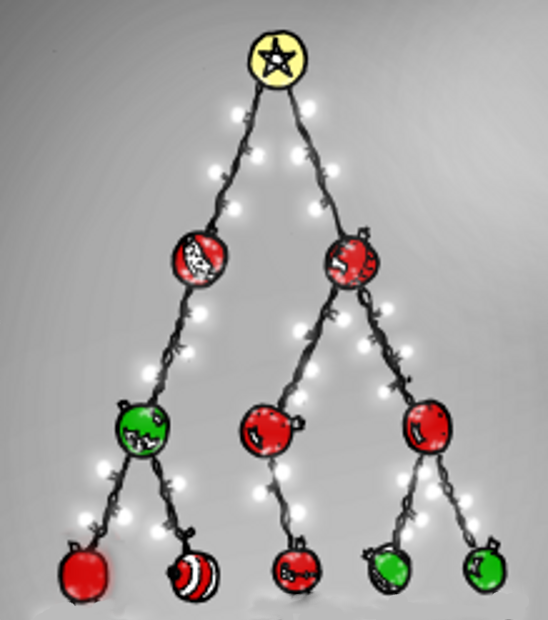
\includegraphics[scale=0.25]{figures/christmas-tree-nothing.png}
\end{frame}

\begin{frame}
\frametitle{How does it figure what to do?}
\hspace{4cm}
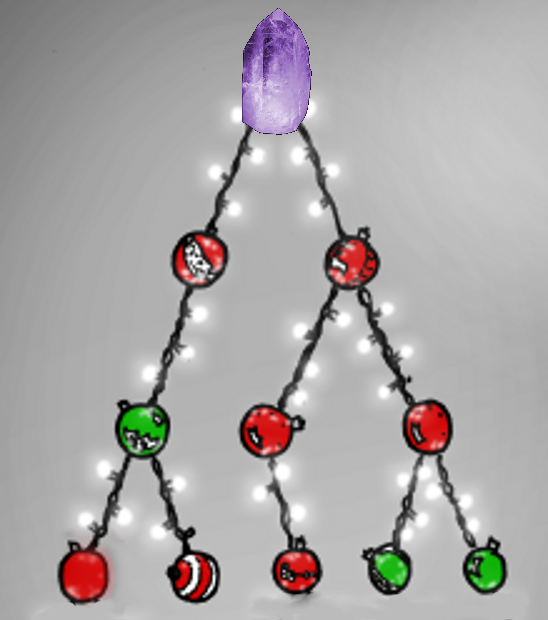
\includegraphics[scale=0.25]{figures/christmas-tree-nothing-crystal.png}
\end{frame}

\begin{frame}
\frametitle{How does it figure what to do?}
\hspace{4cm}
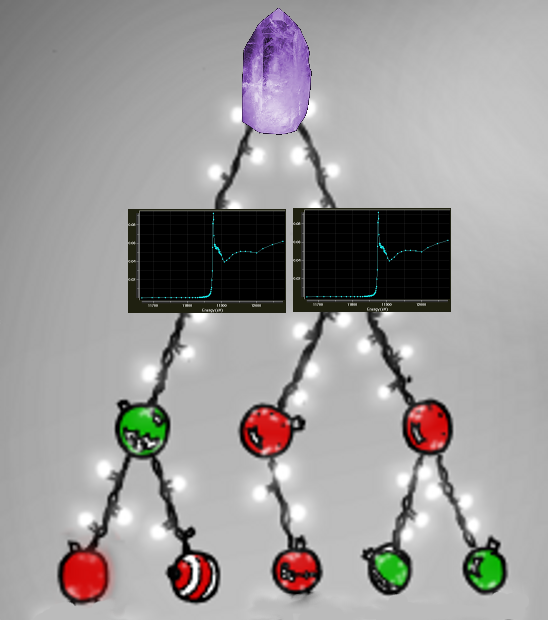
\includegraphics[scale=0.25]{figures/christmas-tree-nothing-wavelength.png}
\end{frame}

\begin{frame}
\frametitle{How does it figure what to do?}
\hspace{4cm}
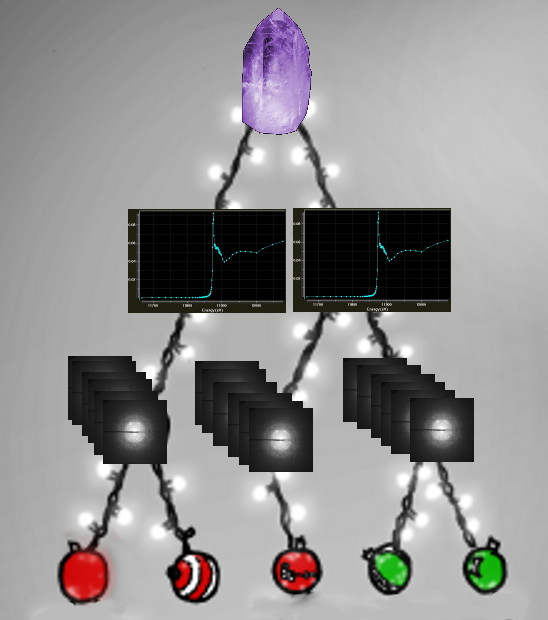
\includegraphics[scale=0.25]{figures/christmas-tree-nothing-sweep.png}
\end{frame}

\begin{frame}[fragile]
\frametitle{What the program sees}
{\small
\begin{verbatim}
BEGIN PROJECT AUTOMATIC
BEGIN CRYSTAL DEFAULT
BEGIN HA_INFO
ATOM Ba
END HA_INFO
BEGIN WAVELENGTH SAD
WAVELENGTH 0.979500
END WAVELENGTH SAD
BEGIN SWEEP SWEEP1
WAVELENGTH SAD
DIRECTORY /dls/i02/data/2011/mx1234-5
IMAGE K5_M1S3_3_001.img
START_END 1 450
END SWEEP SWEEP1
END CRYSTAL DEFAULT
END PROJECT AUTOMATIC
\end{verbatim}
}
\end{frame}

\begin{frame}
\frametitle{Understanding the experiment}
\begin{itemize}
\item{SWEEP: one ``scan'' of images, basic unit of processing}
\item{WAVELENGTH: container of SWEEPs}
\item{WAVELENGTH: all H K L observations merged}
\item{WAVELENGTH: CCP4 MTZ dataset}
\item{CRYSTAL: contains WAVELENGTHs}
\item{CRYSTAL: all data scaled at one}
\end{itemize}
\end{frame}

\begin{frame}
\frametitle{Example: 3QRN\footnote{J.P. Hall et al., Proc. Natl. Acad. Sci. USA 2011 108 (43) 17573-17574}}
\begin{itemize}
\item{Data recorded at Diamond I02}
\item{DNA / ligand complex}
\item{Demonstrates:
\begin{itemize}
\item{Radiation damage}
\item{Heavy atom}
\item{Resolution limits}
\end{itemize}
}
\end{itemize}
\end{frame}

\begin{frame}
\frametitle{Example command line}
{ \huge
xia2 -3d -atom Ba /dls/i02/data/...
}
\end{frame}

\begin{frame}
\frametitle{Example results}
\begin{tabular}{lccc}
High resolution limit      &       \color{red}{1.25} &    6.45 &   1.25\\
Low resolution limit       &                18.85  & 18.85  &  1.27\\
Completeness               &                95.2   & 60.1  &  70.2\\
Multiplicity               &               12.2    & 8.4   &  4.8\\
I/sigma                    &               12.3    & 18.5   &  2.6\\
Rmerge                     &             \color{red}{0.113}  & 
\color{red}{0.096} &  0.564\\
Rmeas(I)                   &             0.129  & 0.118 &  0.633\\
Rmeas(I+/-)                &             0.121  & 0.105 &  0.679\\
Rpim(I)                    &             0.034  & 0.038 &  0.267\\
Rpim(I+/-)                 &             0.043  & 0.041 &  0.368\\
Wilson B factor            &            12.131& & \\
Anomalous completeness     &            93.3  &  52.6  &  58.0\\
Anomalous multiplicity     &           6.4    & 5.0  &   2.0\\
Anomalous correlation      &            0.544 &  0.791 & -0.297\\
Anomalous slope            &      1.085 &  0.000 &  0.000\\
Total observations         &       118588 & 529  &   1634\\
Total unique               &         9749  &  63 &     337\\
\end{tabular}
\end{frame}

\begin{frame}
\frametitle{LogFiles/*aimless.log}
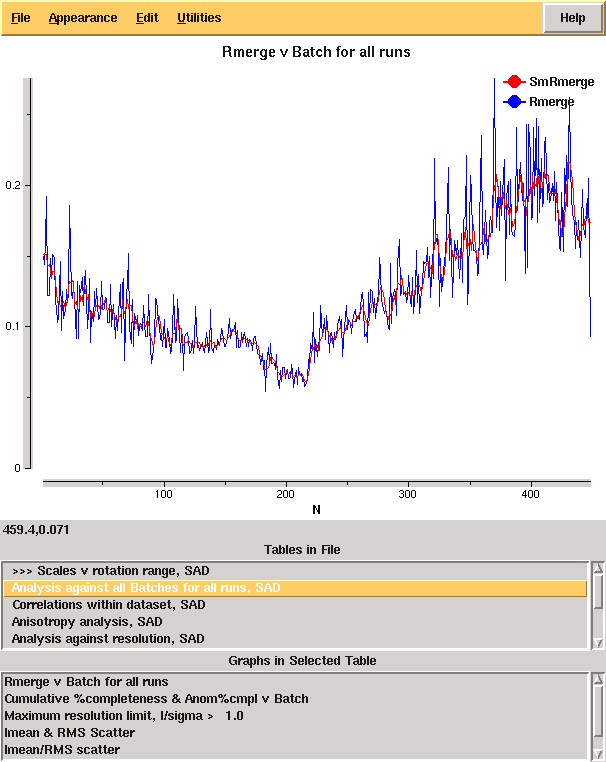
\includegraphics[scale=0.25]{figures/3qrn-all-rmerge-aimless.png}
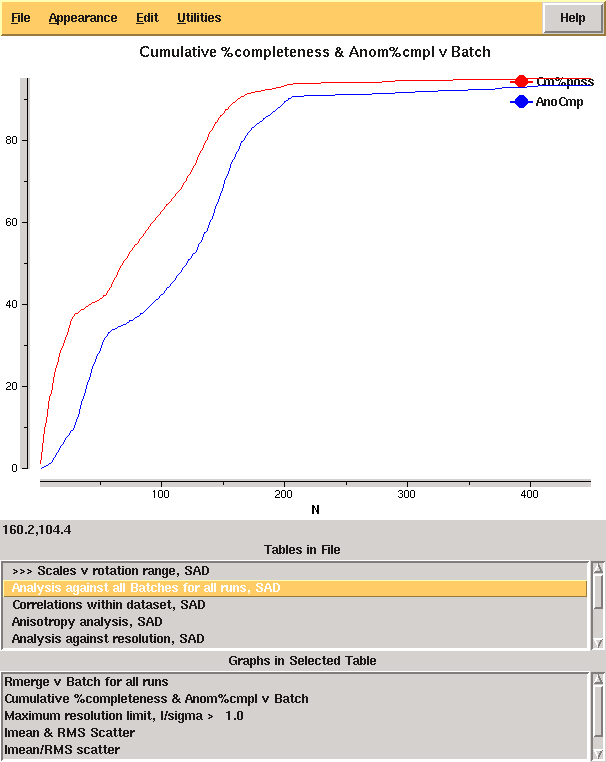
\includegraphics[scale=0.25]{figures/3qrn-all-complete-aimless.png}
\end{frame}

\begin{frame}
\frametitle{What to do next?}
\begin{itemize}
\item{Read automatic.xinfo}
\item{Only process first 200 frames}
\end{itemize}
\end{frame}

\begin{frame}[fragile]
\frametitle{What the program sees}
{\small
\begin{verbatim}
BEGIN PROJECT AUTOMATIC
BEGIN CRYSTAL DEFAULT
BEGIN HA_INFO
ATOM Ba
END HA_INFO
BEGIN WAVELENGTH SAD
WAVELENGTH 0.979500
END WAVELENGTH SAD
BEGIN SWEEP SWEEP1
WAVELENGTH SAD
DIRECTORY /dls/i02/data/2011/mx1234-5
IMAGE K5_M1S3_3_001.img
START_END 1 200 ! THIS WAS 450
END SWEEP SWEEP1
END CRYSTAL DEFAULT
END PROJECT AUTOMATIC
\end{verbatim}
}
\end{frame}

\begin{frame}
\frametitle{Running again}
{ \huge
xia2 -3d -xinfo modified.xinfo
}
\end{frame}

\begin{frame}
\frametitle{Example results II}
\begin{tabular}{lccc}
High resolution limit         &         1.22 &  6.34 &  1.22 \\
Low resolution limit          &        19.62 & 19.62 &  1.24 \\
Completeness                  &         86.9 &  49.1 &  37.8 \\
Multiplicity                  &        5.3  &  4.9   & 1.7 \\
I/sigma                       &        20.1 &  37.0  &  2.3 \\
Rmerge                        &       0.036 & 0.020  &0.355 \\
Rmeas(I)                      &       0.060 & 0.038  &0.448 \\
Rmeas(I+/-)                   &       0.043 & 0.023  &0.491 \\
Rpim(I)                       &       0.023 & 0.014  &0.297 \\
Rpim(I+/-)                    &       0.022 & 0.011  &0.339 \\
Wilson B factor               &       10.70& \\
Anomalous completeness        &        77.7  & 41.0  & 18.3 \\
Anomalous multiplicity        &         2.7  &  3.5  &  0.5 \\
Anomalous correlation         &        0.779 & 0.931 & 0.000 \\
Anomalous slope               &       1.553  &0.000 & 0.000 \\
Total observations            &       50875  &272   & 342 \\
Total unique                  &       9552   &55    & 199 \\
\end{tabular}
\end{frame}

\begin{frame}
\frametitle{Resolution}
\begin{itemize}
\item{Data incomplete at high resolution}
\item{Add RESOLUTION to xinfo file (in either SWEEP or WAVELENGTH}
\item{Add -resolution to the command line}
\end{itemize}
\end{frame}

\section{What did it do?}

\begin{frame}
\frametitle{Indexing}
\begin{itemize}
\item{Initial indexing with LABELIT}
\item{Refine results with XDS indexing}
\item{Use data based on general analysis @ 0, 45, 90 degrees}
\end{itemize}
\end{frame}

\begin{frame}
\frametitle{Indexing}
\hspace{3cm}
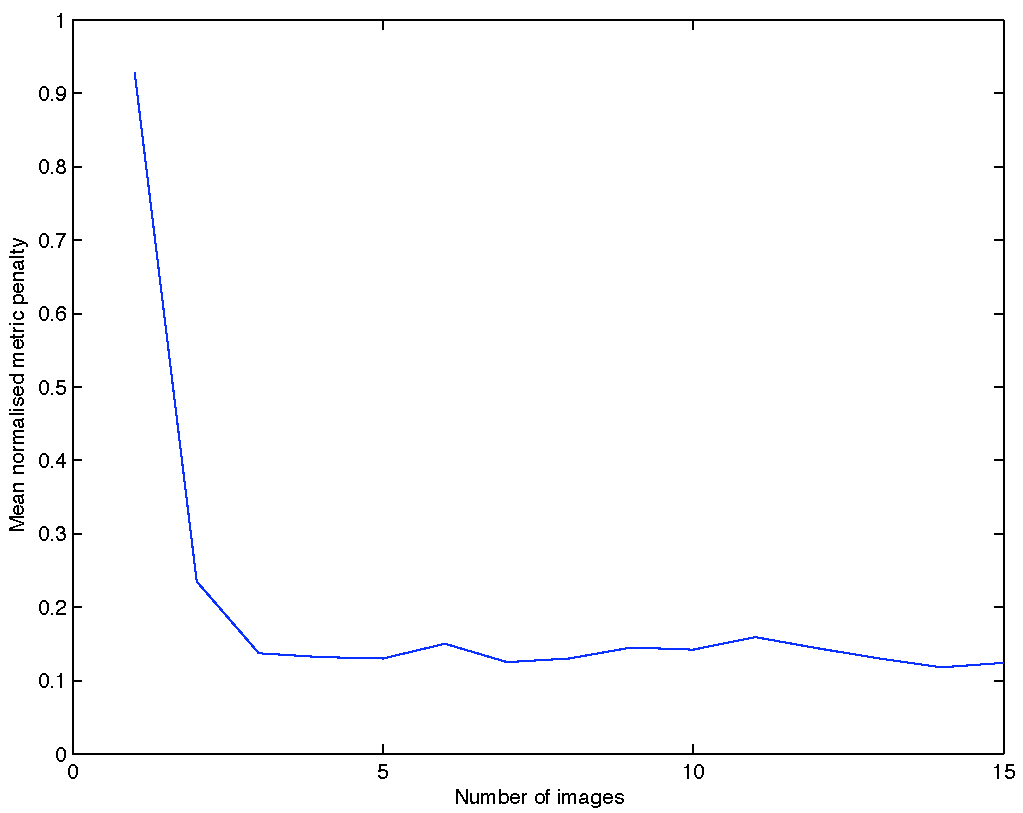
\includegraphics[scale=0.5]{figures/no_images.pdf}
\end{frame}

\begin{frame}
\frametitle{Indexing}
\hspace{3cm}
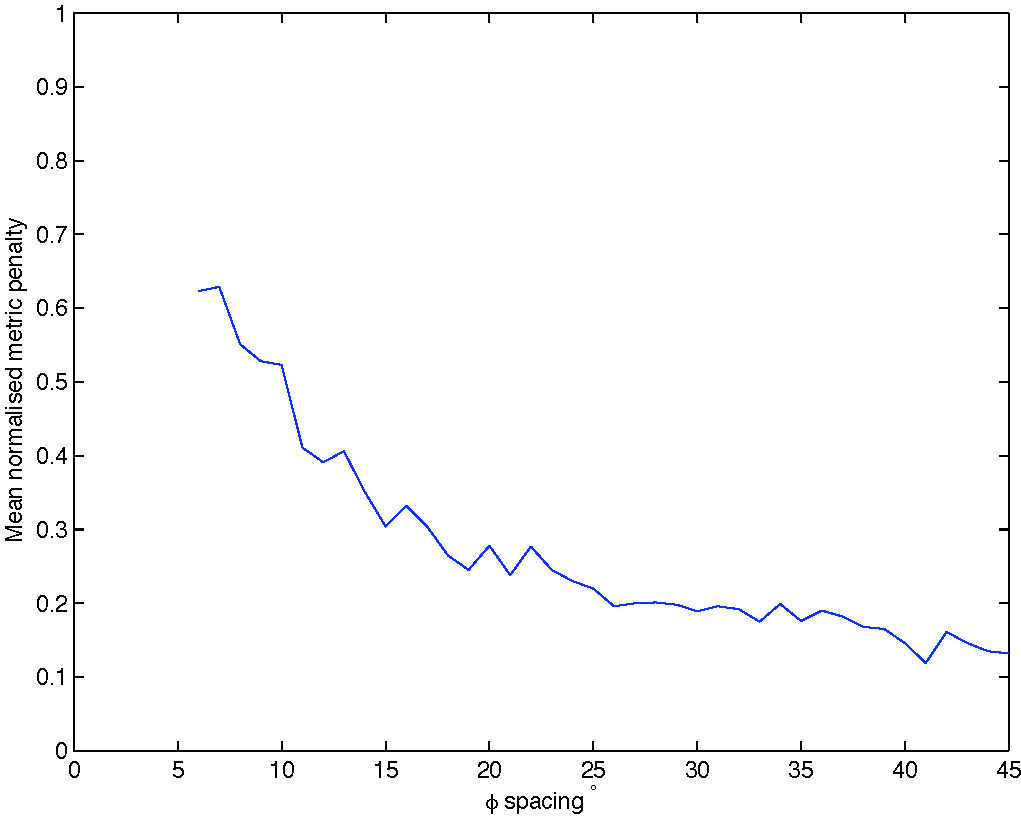
\includegraphics[scale=0.5]{figures/phi_spacing_45a.pdf}
\end{frame}

\begin{frame}
\frametitle{Indexing}
\hspace{3cm}
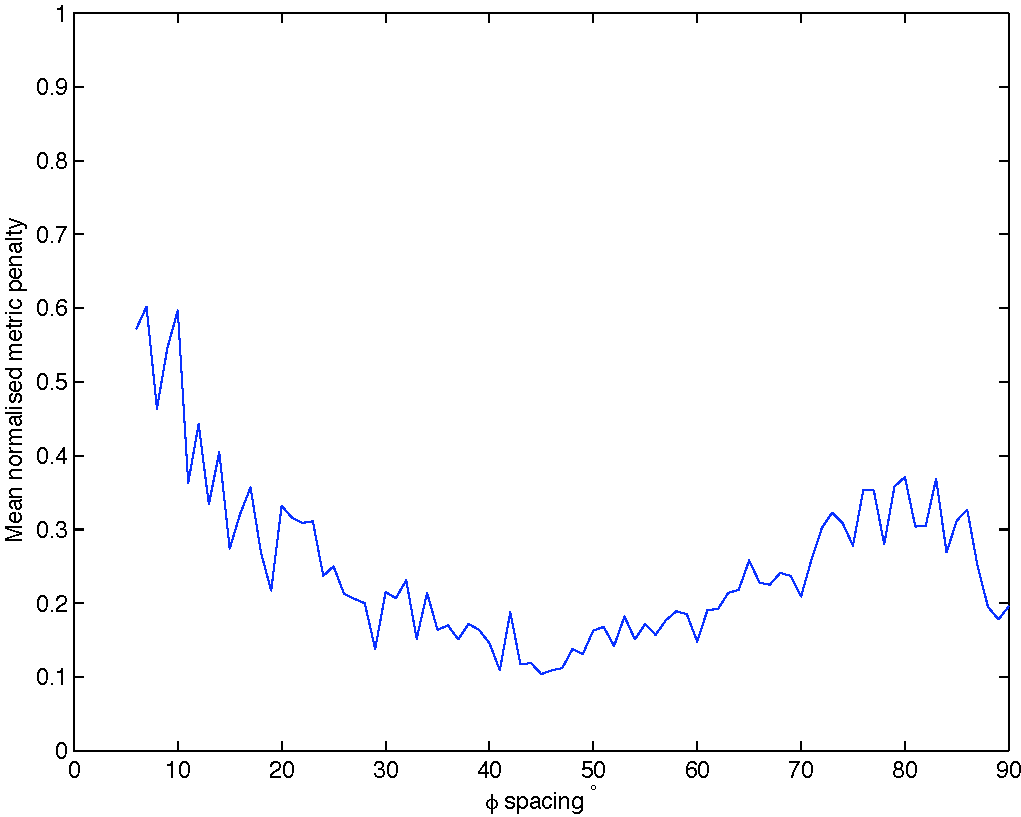
\includegraphics[scale=0.5]{figures/phi_spacing_90a.pdf}
\end{frame}

\begin{frame}
\frametitle{Indexing}
\hspace{6cm}
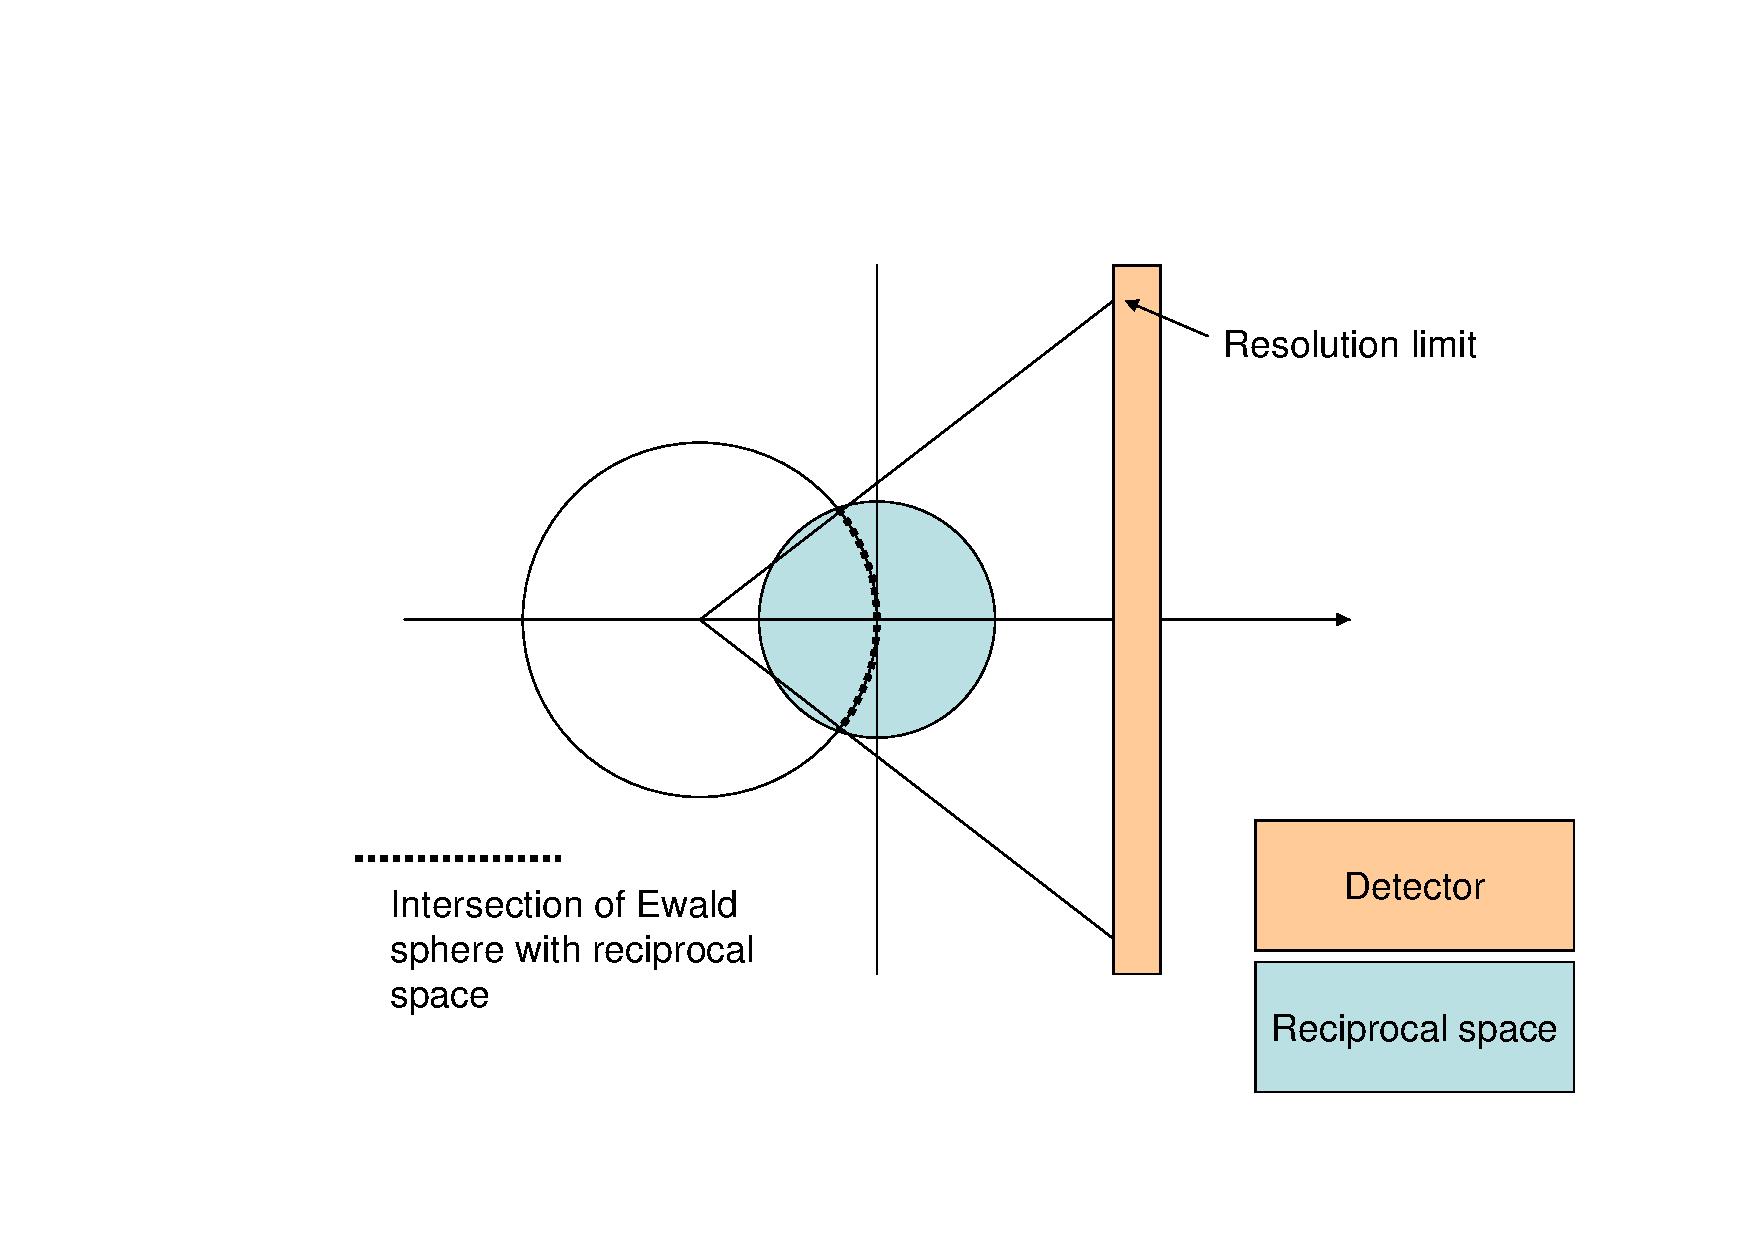
\includegraphics[scale=0.5]{figures/EwaldExplain.pdf}
\end{frame}

\begin{frame}
\frametitle{Indexing}
\hspace{6cm}
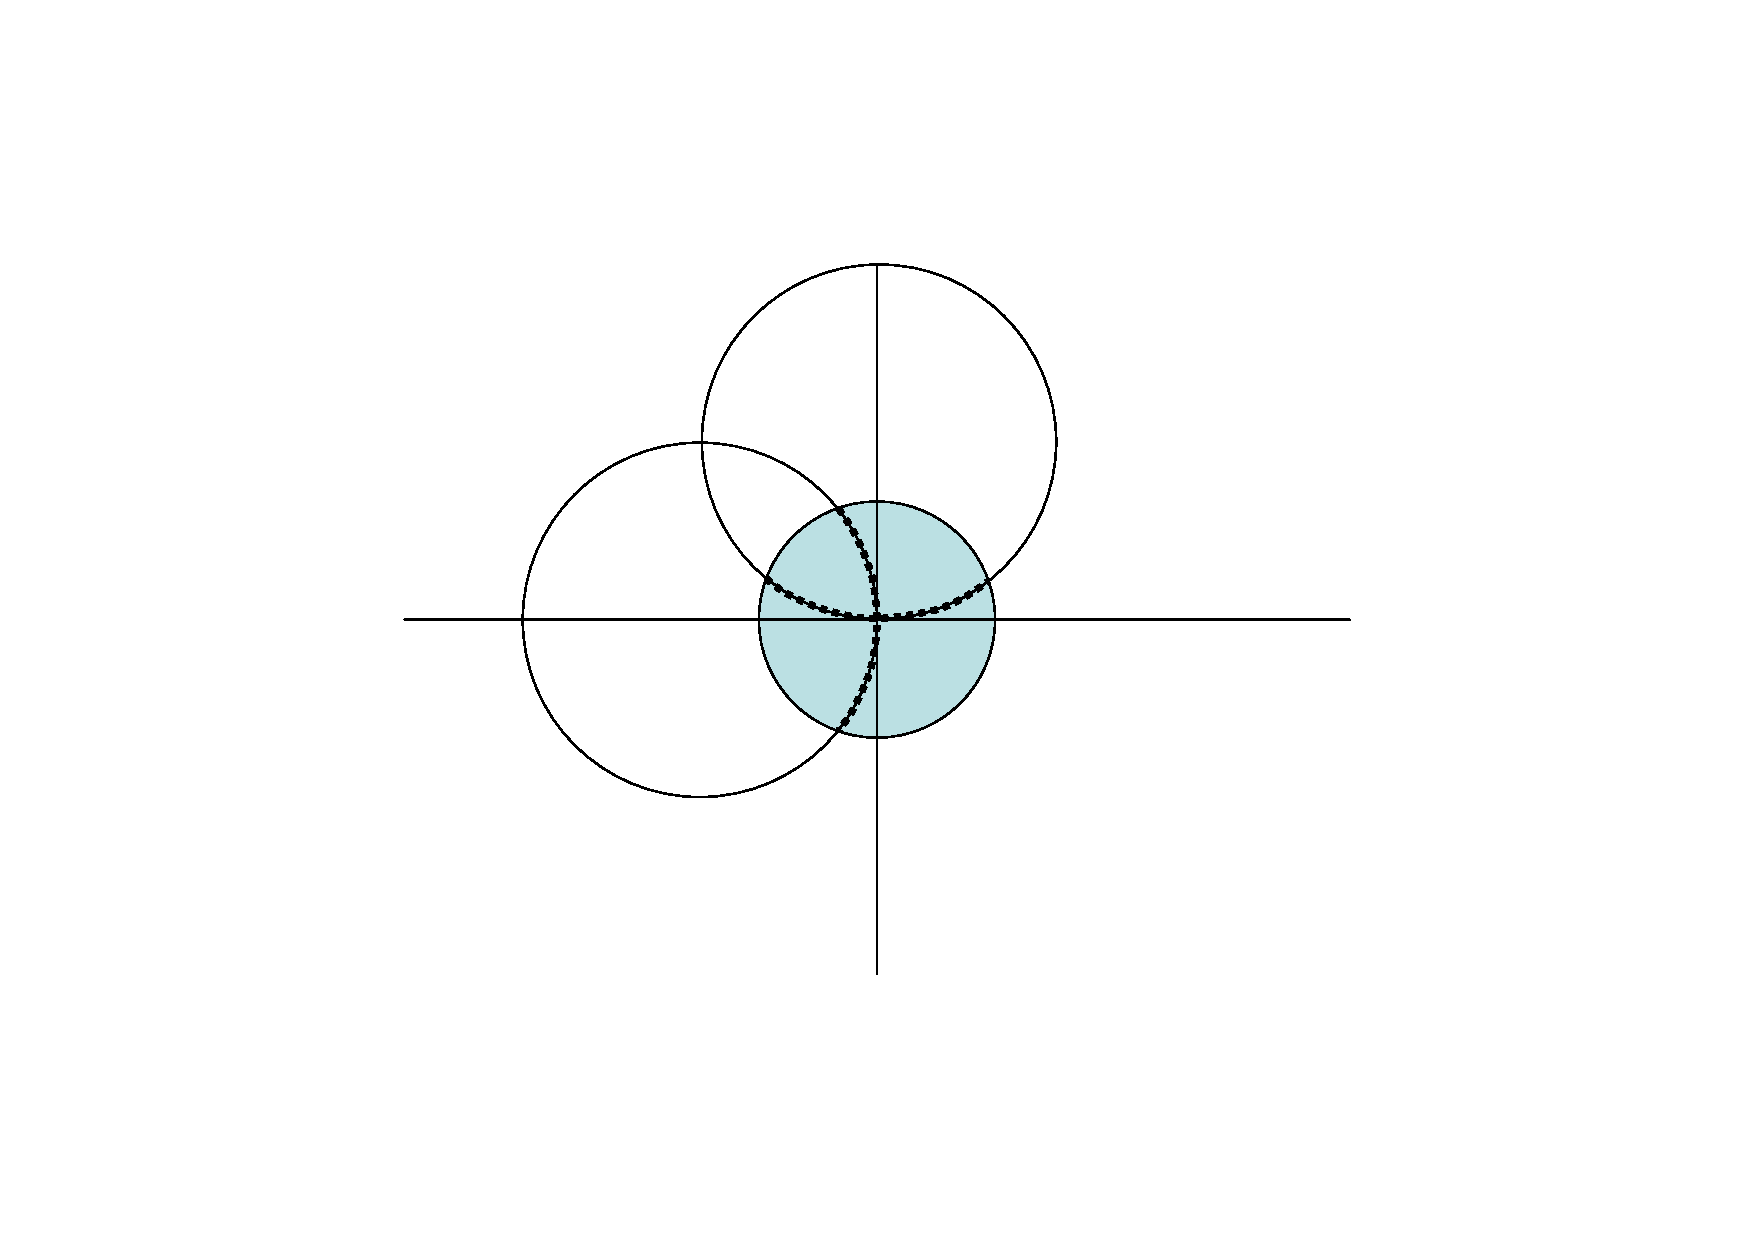
\includegraphics[scale=0.5]{figures/Ewald2Image.pdf}
\end{frame}

\begin{frame}
\frametitle{Indexing}
\hspace{6cm}
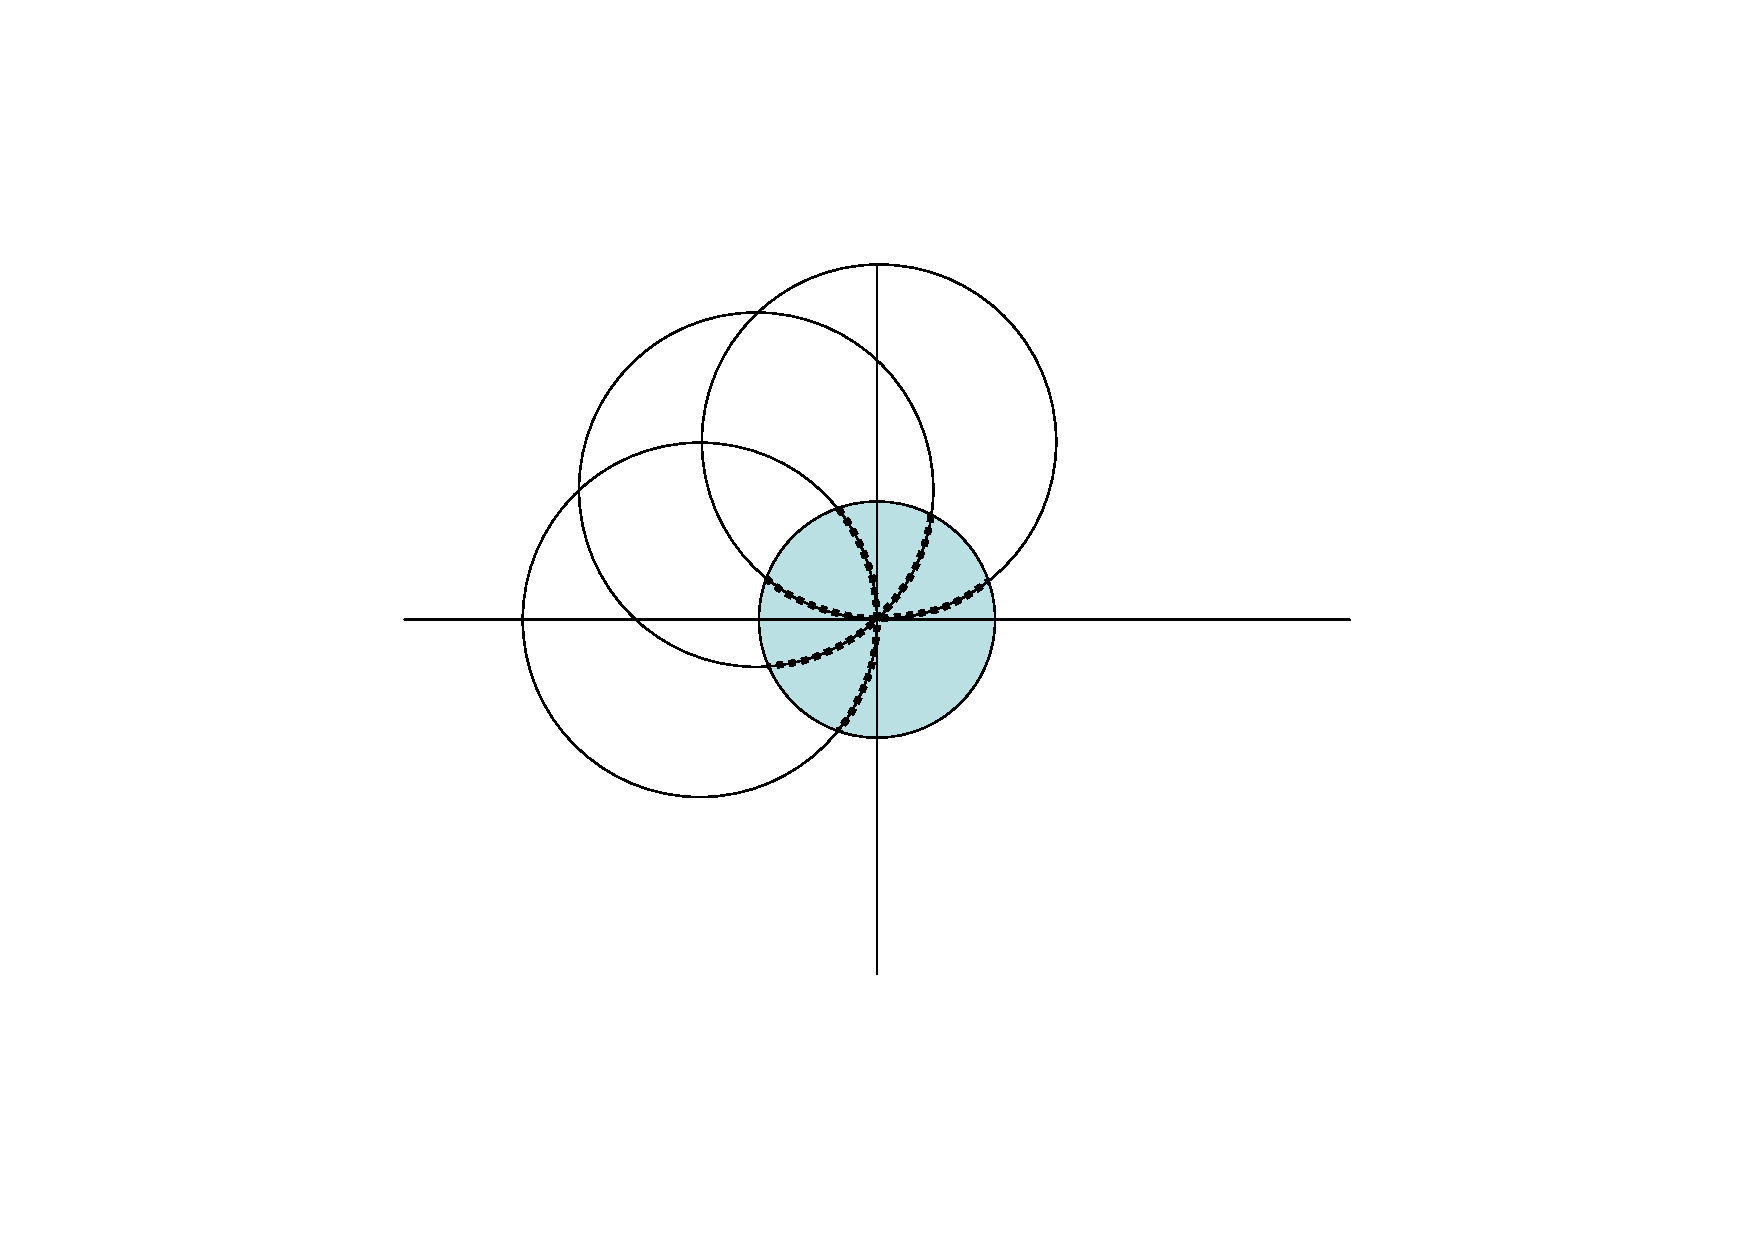
\includegraphics[scale=0.5]{figures/Ewald3Image.pdf}
\end{frame}

\begin{frame}
\frametitle{Integration}
\begin{itemize}
\item{Integrate with lattice constraints applied}
\item{Integrate to corners of detector}
\item{If good reason, repeat integration e.g. with results of postrefinement}
\item{Perform postrefinement in P1, assumed lattice - may reject lattice,
feed back to indexing}
\end{itemize}
\end{frame}

\begin{frame}
\frametitle{Scaling}
\begin{itemize}
\item{Compare results of pointless with remaining allowed lattices:
\begin{itemize}
\item{If agree, proceed}
\item{If lattice not allowed, consider next solution}
\item{If solution lower symmetry than lattice, reject and return to indexing}
\end{itemize}
}
\item{Ensure conclusions consistent}
\item{Ensure consistent setting / origin choice}
\item{Place data into data collection order}
\end{itemize}
\end{frame}

\begin{frame}
\frametitle{Merging}
\end{frame}


\section{What decisions were made?}

\begin{frame}
\frametitle{Resolution limits - default criteria}
\begin{itemize}
\item{Merged $\frac{I}{\sigma_I} > 2$}
\item{Unerged $\frac{I}{\sigma_I} > 1$}
\item{Control with -misigma, -isigma}
\end{itemize}
\end{frame}

\begin{frame}
\frametitle{Resolution limits}
\hspace{6cm}
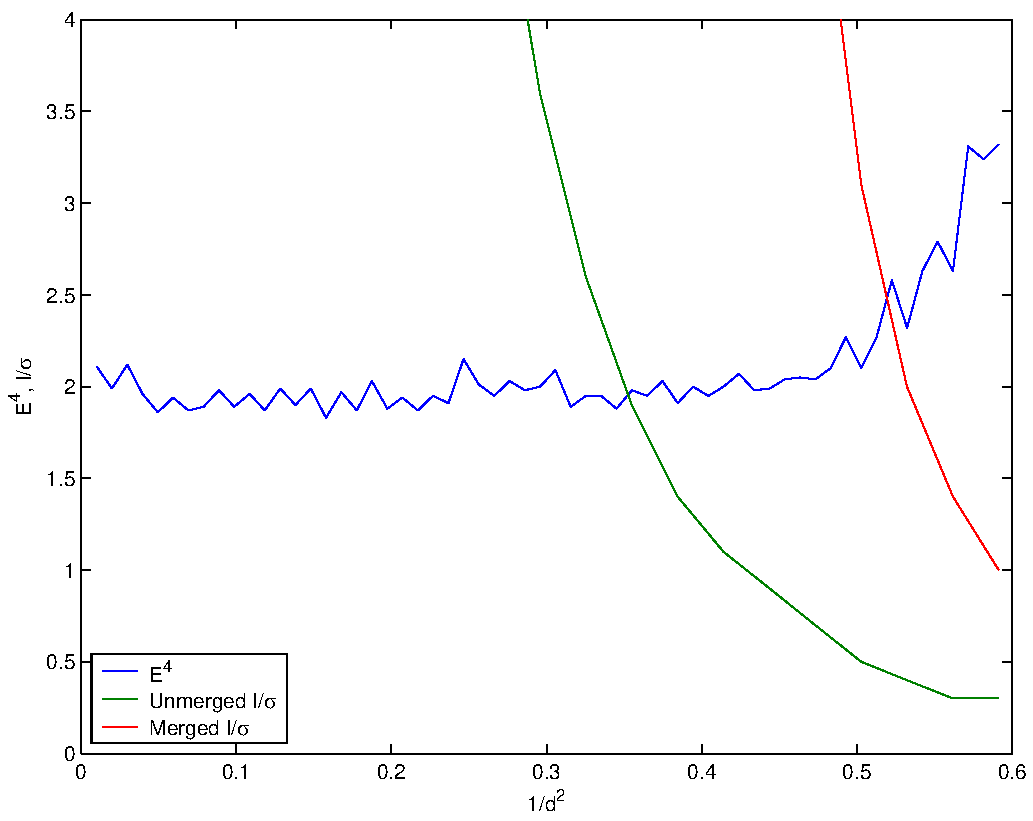
\includegraphics[scale=0.5]{figures/plat-13A-z4.pdf}
\footnote{90-fold multiplicity data from Ed Mitchell @ ESRF}
\end{frame}



\end{document}
